%%% Hlavní soubor. Zde se definují základní parametry a odkazuje se na ostatní části. %%%

%% Verze pro jednostranný tisk:
% Okraje: levý 40mm, pravý 25mm, horní a dolní 25mm
% (ale pozor, LaTeX si sám přidává 1in)
\documentclass[12pt,a4paper]{article}
%\setlength\textwidth{145mm}
\setlength\textheight{247mm}
%\setlength\oddsidemargin{15mm}
%\setlength\evensidemargin{15mm}
\setlength\topmargin{0mm}
\setlength\headsep{0mm}
\setlength\headheight{0mm}
% \openright zařídí, aby následující text začínal na pravé straně knihy
\let\openright=\clearpage

%% Pokud tiskneme oboustranně:
% \documentclass[12pt,a4paper,twoside,openright]{report}
% \setlength\textwidth{145mm}
% \setlength\textheight{247mm}
% \setlength\oddsidemargin{15mm}
% \setlength\evensidemargin{0mm}
% \setlength\topmargin{0mm}
% \setlength\headsep{0mm}
% \setlength\headheight{0mm}
% \let\openright=\cleardoublepage

%% Pokud používáte csLaTeX (doporučeno):
\usepackage{czech}
%% Pokud nikoliv:
%\usepackage[czech]{babel}
%\usepackage[T1]{fontenc}

%% Použité kódování znaků: obvykle latin2, cp1250 nebo utf8:
\usepackage[utf8]{inputenc}

%% Ostatní balíčky
\usepackage{graphicx}
\usepackage{tikz}
\usepackage{tikz-3dplot}

\usetikzlibrary{patterns}
\usetikzlibrary{decorations.pathreplacing}

\usepackage{mathtools}
\usepackage{listings}

\usepackage{amsthm}
\usepackage{amssymb}

\usepackage{needspace}

\newenvironment{priklad}{%
    \par%
    \vspace{1em}%
    \leftskip=2\parindent
    \rightskip=2\parindent
    \small
    \needspace{3\baselineskip}
    \begin{sloppypar}%
    \noindent\textit{\textbf{Příklad.}}%
}{%
    \end{sloppypar}%
    \vspace{1em}%
}

\usepackage{array}
\newcolumntype{t}{>{\tt}}

\usepackage[disable, textsize=tiny]{todonotes}
\usepackage[bottom, hang]{footmisc}

\usepackage{caption}
\usepackage[noend]{algpseudocode}
\usepackage{algorithm}
\floatname{algorithm}{Algoritmus}

\newcommand{\var}[1]{\textit{#1}}
\newcommand{\func}[2]{\mbox{\textsc{#1}}\ifx&#2&\else(#2)\fi}
\newcommand{\keyword}[1]{\textbf{#1}}
\newcommand{\NULL}{{\small NULL }}

\newcommand{\class}[1]{\texttt{#1}}
\newcommand{\method}[2]{\texttt{\mbox{#1}\ifx&#2&()\else(#2)\fi}}
\newcommand{\function}[2]{\texttt{\mbox{#1}\ifx&#2&()\else(#2)\fi}}

\usepackage{alltt}

%\usepackage{showframe}

%% Balíček hyperref, kterým jdou vyrábět klikací odkazy v PDF,
%% ale hlavně ho používáme k uložení metadat do PDF (včetně obsahu).
%% POZOR, nezapomeňte vyplnit jméno práce a autora.
%\usepackage[ps2pdf,unicode]{hyperref}   % Musí být za všemi ostatními balíčky
\usepackage[unicode]{hyperref}   % Musí být za všemi ostatními balíčky
\hypersetup{
    colorlinks,%
    citecolor=black,%
    filecolor=black,%
    linkcolor=black,%
    urlcolor=black
}
\hypersetup{pdftitle=Ovládání počítače pomocí jednobarevných objektů snímaných
kamerou - Uživatelská dokumentace}
\hypersetup{pdfauthor=Richard Jedlička}

\usepackage[all]{hypcap}

\newenvironment{itemize_compact}{\begin{list}{$\bullet$}{
    \setlength{\parsep}{0mm}
    \setlength{\itemsep}{0mm}
}}{\end{list}}%

\newcommand{\sectionline}{%
  %\nointerlineskip 
  %\vspace{\baselineskip}%
  \begin{center}
  \noindent\rule{\linewidth}{.5pt}%
  \end{center}
  %\par\nointerlineskip
  %\par% \vspace{\baselineskip}
}

\usepackage{glossaries}
\usepackage{xkeyval}
\usepackage{xstring}

\makeatletter

\newcommand{\termdef}[2]{%
    \csname term@#1@#2\endcsname%
}

\newcommand{\newterm}[2]{%
    \define@cmdkeys{term}[term@#1@]{%
        description,plural,sort,see,%
        1pad,2pad,3pad,4pad,5pad,6pad,7pad%
    }[none]
    \setkeys{term}{#2}
    \newglossaryentry{#1}{%
        name={\termdef{#1}{1pad}},%
        description={\termdef{#1}{description}},%
        plural={\termdef{#1}{plural}},%
        sort={\termdef{#1}{sort}},%
        see={\termdef{#1}{see}},%
        first={\itshape\termdef{#1}{1pad}}%
    }
}

\newcommand{\term}[2][1pad]{%
    \IfEq{#1}{1pad}{%
        \gls{#2}%
    }{%
        \glslink{#2}{\termdef{#2}{#1}}%
    }%
}

\newcommand{\Term}[2][1pad]{%
    \IfEq{#1}{1pad}{%
        \Gls{#2}%
    }{%
        \Glslink{#2}{\termdef{#2}{#1}}%
    }%
}

\makeatother

%%% Drobné úpravy stylu

% Tato makra přesvědčují mírně ošklivým trikem LaTeX, aby hlavičky kapitol
% sázel příčetněji a nevynechával nad nimi spoustu místa. Směle ignorujte.
%\makeatletter
%\def\@makechapterhead#1{
  %{\parindent \z@ \raggedright \normalfont
   %\Huge\bfseries \thechapter. #1
   %\par\nobreak
   %\vskip 20\p@
%}}
%\def\@makeschapterhead#1{
  %{\parindent \z@ \raggedright \normalfont
   %\Huge\bfseries #1
   %\par\nobreak
   %\vskip 20\p@
%}}
%\makeatother

% Toto makro definuje kapitolu, která není očíslovaná, ale je uvedena v obsahu.
%\def\chapwithtoc#1{
%\chapter*{#1}
%\addcontentsline{toc}{chapter}{#1}
%}

\linespread{1.3}

\clubpenalty 10000
\widowpenalty 10000

\usepackage{encxvlna}
\begin{document}

% Trochu volnější nastavení dělení slov, než je default.
%\lefthyphenmin=2
%\righthyphenmin=2

%%% Titulní strana práce

\pagestyle{empty}
\begin{center}

\large

%\centerline{\mbox{\includegraphics[width=60mm]{img/logo.pdf}}}

%\vspace{5mm}

\vspace*{3cm}

% Název práce přesně podle zadání
{\LARGE\bfseries Ovládání počítače pomocí jednobarevných objektů snímaných kamerou}

\vfill

{\Huge Uživatelská dokumentace}
% Název katedry nebo ústavu, kde byla práce oficiálně zadána
% (dle Organizační struktury MFF UK)

\vfill

{\large Richard Jedlička}

\vfill

% Zde doplňte rok
2012

\end{center}

\newpage

%%% Následuje vevázaný list -- kopie podepsaného "Zadání bakalářské práce".
%%% Toto zadání NENÍ součástí elektronické verze práce, nescanovat.

%%% Na tomto místě mohou být napsána případná poděkování (vedoucímu práce,
%%% konzultantovi, tomu, kdo zapůjčil software, literaturu apod.)

\openright

\newpage

%%% Strana s automaticky generovaným obsahem bakalářské práce. U matematických
%%% prací je přípustné, aby seznam tabulek a zkratek, existují-li, byl umístěn
%%% na začátku práce, místo na jejím konci.

\openright
\pagestyle{plain}
\setcounter{page}{1}
\tableofcontents

\thispagestyle{empty}

%%% Jednotlivé kapitoly práce jsou pro přehlednost uloženy v samostatných souborech

\newpage

\section{Systémové požadavky}
Aplikace ke svému běhu potřebuje počítač nainstalovaným operačním systémem
\textbf{GNU/Linux}. Dále vyžaduje funkční \textbf{webovou kameru}. Processor
alespoň \textbf{1.6GHz} (v této konfiguraci sice není ovládání příliš plynulé,
ale je použitelné).

\section{Softwarové závislosti}
Aplikace využívá některé knihovny a frameworky, které je potřeba mít
nainstalované v systému, aby bylo možné zkompilovat a spustit.

\begin{itemize}
    \item \textbf{Qt Framework 4.8}\\
    \url{http://qt.nokia.com}
    \item \textbf{Boost 1.49.0}\\
    \url{http://www.boost.org}
    \item \textbf{Xlib} \\
    \url{http://www.x.org}
    \item \textbf{libv4l2} \\
    \url{http://linuxtv.org}
\end{itemize}

\section{Sestavení a instalace}
Pro sestavení aplikace je potřeba mít tyto nástroje:

\begin{itemize}
    \item \textbf{Make} \\
    \url{http://www.gnu.org/software/make/}
    \item \textbf{pkg-config} \\
    \url{http://www.freedesktop.org/wiki/Software/pkg-config}
    \item \textbf{GCC 4.7.0} (byli použity konstrukce ze standardu C++11) \\
    \url{http://gcc.gnu.org/}
\end{itemize}

\bigskip\noindent
Dále zmiňované projekty naleznete na přiloženém CD. Před sestavením, je třeba
projekty zkopírovat mimo CD do nějaké zapisovatelné složky.

\bigskip\noindent
Nejprve je potřeba sestavit a nainstalovat \textbf{FakeInput} a
\textbf{Gecon Framework}.

Posloupnost příkazů příkazové řádky pro sestavení je následující:

\begin{quote}
\texttt{> cd <složka-projektu>}\\
\texttt{> make config=release}
\end{quote}

FakeInput a Gecon Framework je třeba nainstalovat aby byli vyhledatelné v
systému. Buď se nainstalují přímo do standardních instalačních cest v systému,
nebo je možné využít \uv{vývojářské} instalace, která nainstaluje soubory v
rámci projektové složky.

Standardní instalace:
\begin{quote}
\texttt{> make install intall\_prefix=<prefix-pro-instalaci>}
\end{quote}

\uv{Vývojářská} instalace:
\begin{quote}
\texttt{> make dev-install}
\end{quote}

Pokud se projekty nainstalují pomocí \uv{vývojářské} instalace nebo do
nestandardní cesty, je třeba přidat instalační cesty do proměnných prostředí:

\begin{quote}
\small
\texttt{> LD\_LIBRARY\_PATH=\$LD\_LIBRARY\_PATH:<prefix-FakeInput>/lib}\\
\texttt{> LD\_LIBRARY\_PATH=\$LD\_LIBRARY\_PATH:<prefix-GeconFramework>/lib}\\
\texttt{> export LD\_LIBRARY\_PATH}
\end{quote}
\begin{quote}
\small
\texttt{>
    PKG\_CONFIG\_PATH=\$PKG\_CONFIG\_PATH:<prefix-FakeInput>/lib/pkgconfig}\\
\texttt{>
    PKG\_CONFIG\_PATH=\$PKG\_CONFIG\_PATH:<prefix-GeconFramework>/lib/pkgconfig}\\
\texttt{> export PKG\_CONFIG\_PATH}
\end{quote}

\texttt{<prefix-FakeInput>} a \texttt{<prefix-GeconFramework>} jsou prefix
nastavené při instalaci, v případě \uv{vývojářské} instalace jsou to složky
projektů.

\bigskip
Nyní je možné sestavit \textbf{Gecon PC}.
\begin{quote}
\texttt{> cd <složka-GeconPC>}\\
\texttt{> make config=release}
\end{quote}

Aplikaci spustíme pomocí \texttt{make run}.

\section{Práce s aplikací}
V této sekci popíšeme, jak se pracuje s aplikací. Hlavní okno programu vypadá
jako na obrázku \ref{fig:mainwindow}.

\begin{figure}[h]
\centering
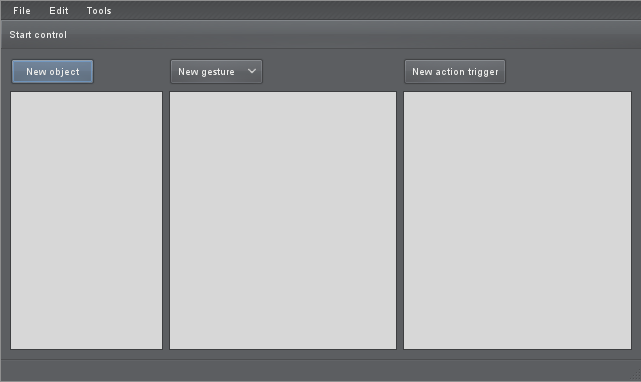
\includegraphics[width=\textwidth]{mainwindow.png}
\caption{Hlavní okno}
\label{fig:mainwindow}
\end{figure}

Je rozděleno na tři části: část pro objekty (vlevo), část pro gesta
(uprostřed) a část pro spoštěče akcí (vpravo).

Panel pod nabídkou menu obsahuje tlačíto \emph{Start control}, které spouští
kontrolní cyklus ovládání. Před spuštěním je ale potřeba přidat objekty, gesta
a spouštěče akcí.

\subsection{Nastavení webové kamery}
Pokud je k počítači připojeno více webových kamer, tu správnou si vyberete
pomocí dialogu nastavení \emph{Settings}. Nachází se v nabídce \emph{Edit}.

\begin{figure}[h]
\centering
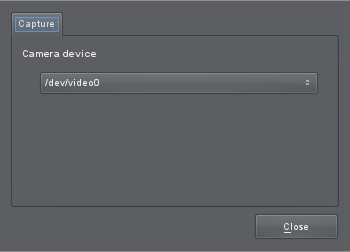
\includegraphics[width=0.7\textwidth]{settings.png}
\caption{Výběr webové kamery}
\label{fig:settings}
\end{figure}

Pokud nejsou k dispozici žádná zařízení, aplikace o tom dá vědět varovnou
hláškou. V tom případě bude aplikace dále fungovat, jen nebude funkční vše co
pracuje se snímky z kamery (tedy práce s objekty, s pohybovými gesty a samotné
ovládání).

\subsection{Práce s objekty}
Nový objekt se přidává před dialog, který se aktivuje kliknutím na tlačítko
\emph{New object}. Dialog je vyobrazen na obrázku \ref{fig:newobject}. Uprostřed je zobrazeno
video snímané kamerou. Pro získání barvy objektu, je třeba umístit objekt, tak
aby byl vidět v záběru a po té na něj kliknout. Detekovaný objekt pak bude
vyznačen oblastí vyplněnou modrými tečkami a zeleným konvexním obalem a
červeným opsaným obdélníkem.

Pokud se bude vyznačena jiná oblast, než jste očekávali, zkuste kliknout do
různým míst v objektu. Pokud ani to nepomůže, je buď špatné osvětlení, barva
objektu je málo výrazná nebo se v pozdaní nachází příliš podobný objekt.

\begin{figure}[h]
\centering
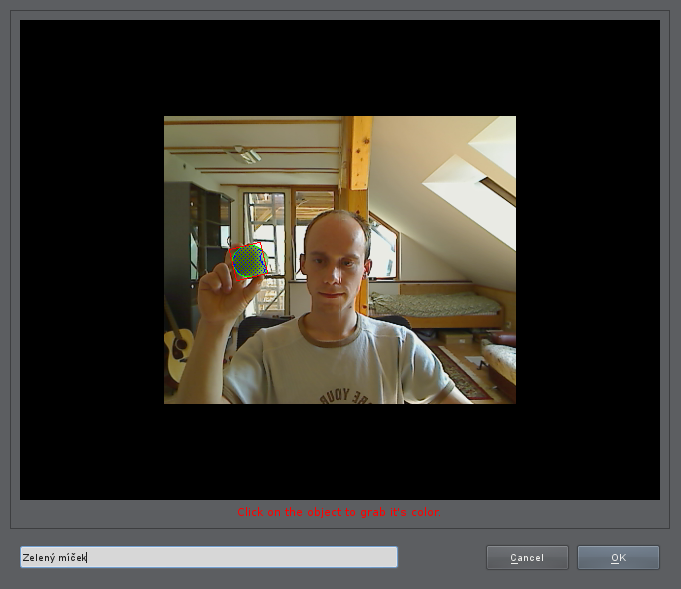
\includegraphics[width=\textwidth]{newobject.png}
\caption{Dialog pro přidání nového objektu}
\label{fig:newobject}
\end{figure}

Objekty vybírejte s pokud možno co nejsytější barvou. Osvětlení je vhodné
čelní, nikoli však přímé. Jako vhodné se ukálazo sedět proti oknu (samozřejmě
ne s přímým sluncem) nebo sedět proti stěně a namířit na ni rozsvícenou
lampičku.

Po vyznačení objektu s ním zkuste pohybovat, natáčet ho, oddalovat i
přibližovat, abyste zjistili, zda bude správně vyznačen i v jiných místech
záběru. Také zkuste objektem vyjet mimo záběr, ideální je, pokud poté nedojde k
označení jiného objektu. Pokud vyznačení nevyhovuje, opět zkuste klikat na
různá místa v objektu (světlejší, tmavší).

Dialog obsahuje pole pro název objektu. Pokud ho necháte prázdné, aplikace
vybere vhodný unikátní identifikátor.

Jakmile jste s vyznačením objektu spokojeni, klikněte na \emph{OK}. Pokud je
vše v pořádku, objekt se přidá a bude zobrazen v hlavním okně. Můžou ale
nastat dvě komplikace, které Vám aplikace oznámí. Pokud se pokusíte přidat
objekt bez jeho vyznačení, nebo jste již velmi podobný objekt přidali dříve.

\begin{figure}[h]
\centering
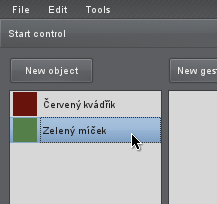
\includegraphics[width=0.5\textwidth]{object.png}
\caption{Zobrazení objektu v hlavním okně}
\end{figure}

Pro úpravu objektu klikněte dvakrát na jeho zobrazení v hlavním okně. Tím
otevřete stejný dialog jako při přidávání objektu a úprava objektu probíhá
také stějně jako přidávání.

Jediné co se v dialogu objeví navíc je tlačítko
\emph{Delete}, kterým můžete objekt smazat. 

\subsection{Práce s gesty}

\begin{figure}[h]
\centering
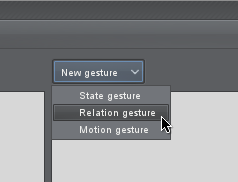
\includegraphics[width=0.5\textwidth]{newgesturemenu.png}
\caption{Menu pro výběr typu gesta pro přidání}
\label{fig:newgesturemenu}
\end{figure}

Pro práci s gesty slouží prostřední část hlavního okna. Pro přidání nového
gesta klikněte na tlačítko \emph{New gesture}. Vyjede menu, kde si vybere jaké
gesto chcete přidat (viz obrázek \ref{fig:newgesturemenu}). Jsou na výběr tři
typy gest -- stavové, vztahové a pohybové.

Začneme \textbf{stavovým gestem}. Dialog nového stavového gesta umožňuje nastavit
podmínku, kterou musí splňovat vlastnost objektu. Dialog obsahuje několik
rozbalovacích seznamů. Jednotlivé prvky jsou za sebou poskládány tak, aby šlo
podmínku stavět inutivně jako větu. Na prvním místě je výběr objektu, za ním
vlastnost, dále následuje relace která se vztahuje k hodnotě na posledním
místě. Prvky pro výběr relace a hodnoty se mění podle vybrané vlastnosti
objektu.

\begin{figure}[h]
\centering
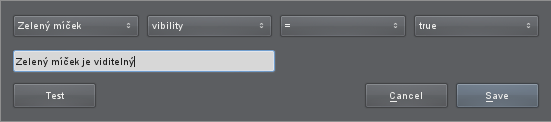
\includegraphics[width=1.1\textwidth]{newstategesture.png}
\caption{Dialog pro přidání nového stavového gesta}
\label{fig:newstategesture}
\end{figure}

Vlastnosti na výběr jsou:
\begin{itemize_compact}
    \item \emph{viditelnost}
    
    Porovnává se vůči pravdivostní hodnotě \emph{prava/nepravda}, ve smyslu
    \emph{je~viditelný / není~viditelný}. Obrázek \ref{fig:newstategesture}
    ukazuje nastavení podmínky na \uv{objekt je viditelný}.

    \item \emph{pozice}

    Porovnává se vůči jiné pozici. Souřadnice pozice se zadávají v procentech.
    Relace na výběr jsou \emph{nad/pod} pozicí, \emph{nalevo/napravo}
    od pozice a \emph{blíže/dále} než zadaná vzdálenost od pozice.

    \item \emph{sklon}\nopagebreak

    Sklon se porovnává s číselnou hodnotou zadanou v úhlech. Hodnota úhlu má
    smysl v rozmezí 0--179$^{\circ}$.

    \item \emph{obsah}

    Obsah se porovnává s hodnotu zadanou zlomkem. Zlomek určuje, jakou část
    snímku objekt zbírá.

    \item \emph{poměr stran}

    Poměr stran se porovnává s číselnou reálnou hodnotou, vyjadřují podíl
    \emph{delší strana} $/$ \emph{kratší strana}.
\end{itemize_compact}

\begin{figure}[h]
\centering
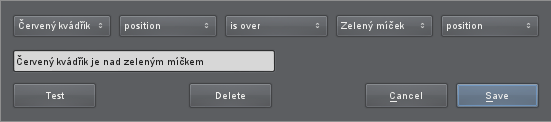
\includegraphics[width=1.1\textwidth]{newrelationgesture.png}
\caption{Dialog pro přidání nového vztahového gesta}
\label{fig:newrelationgesture}
\end{figure}

\textbf{Vztahové gesto} se zadává velmi podobně. Jediný rozdíl je v tom, že
místo prvků pro zadání konkrétní hodnoty jsou zde prvky pro zadání vlastnosti
druhého objektu.

\begin{figure}[h]
\centering
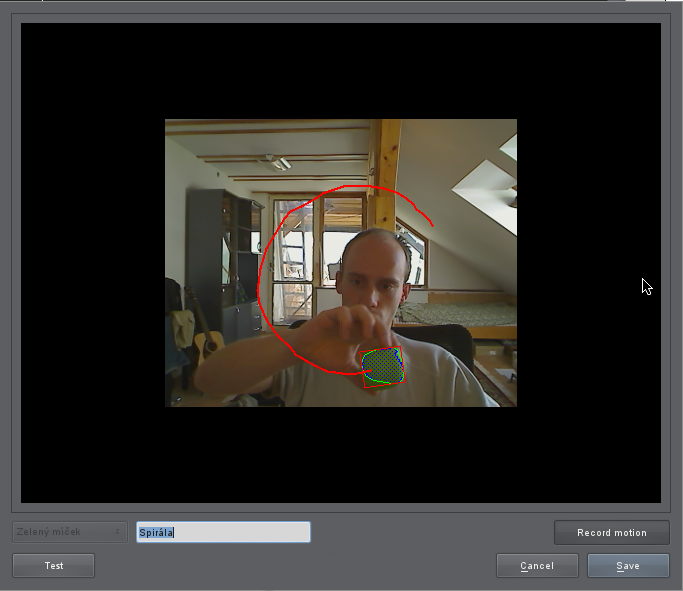
\includegraphics[width=0.9\textwidth]{newmotiongesture1.png}
\caption{Zaznamenávání trajektorie pohybu objektu}
\label{fig:newrelationgesture1}
\end{figure}

Zadávání nového \textbf{pohybového gesta} se naopak úplně liší. Dialog slouží
k zaznamenání trajektorie pohybu objektu. Nejprve vyberte objekt (vlevo dole),
pro který chcete zaznamenat gesto. Pak stiskněte tlačítko \emph{Record
motion}, tím se spustí video, ale ještě neprobíhá zaznamenávání. Přípravte si
objekt na pozici, odkud chcete pohyb začít, a až budete připraveni, klikněte na
\emph{Ready}. Nyní pohybujte objektem. Až dokončíte pohyb, držte objekt na
jednom místě. Aplikace rozpozná, že jste dokončili pohyb přestane dále
zaznamenávat. Poté zaznamenanou trajektorii zobrazí.

\begin{figure}[h]
\centering
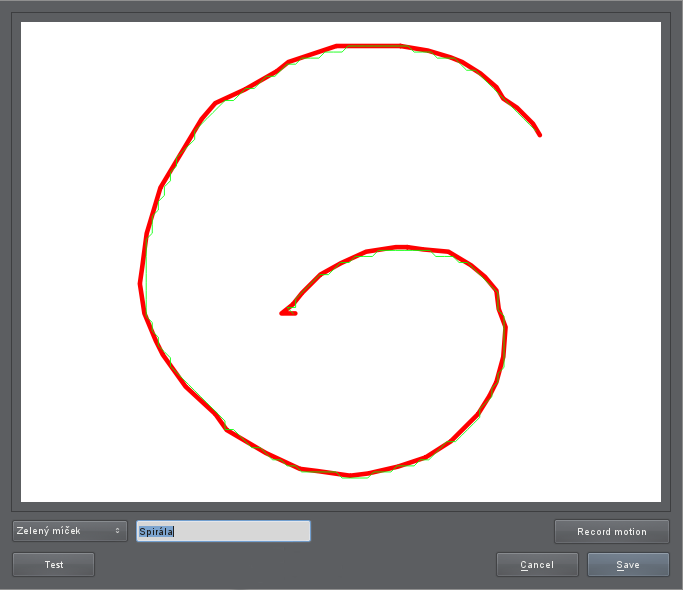
\includegraphics[width=0.9\textwidth]{newmotiongesture2.png}
\caption{Zaznamenávání trajektorie pohybu objektu}
\label{fig:newrelationgesture2}
\end{figure}

Pokud pohyb bude mít příliš malý rozhas pozic, nebo zaznamenán. Je potřeba aby
rozsah krajních bodů (levého a pravého nebo horního a dolního), byl alespoň
čtvrtina šírky snímku.

Pokud chcete zaznamenat gesto znovu, opakujte postup popsany výše.

Nyní lze zaznamenaou pozici uložit tlačítkem \emph{Save}. Pokud jste již dříve
uložili gesto, které je hodně podobné nově zaznamenanému, aplikace ho odmítne
uložit.

\bigskip
Všem gestů je možné nastavit název, pokud ho ale neuvedete, tak jako u objektů
aplikace vybere vhodný unikátní identifikátor.

\begin{figure}[H]
\centering
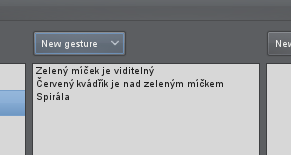
\includegraphics[width=0.7\textwidth]{gestures.png}
\caption{Uložená gesta}
\label{fig:gestures}
\end{figure}

\bigskip
Uložená gesta se pak zobrazí v hlavním okně, v pořadí stavová gesta, vztahová
gesta a nakonec pohybová gesta.

Gesta je možné upravit dvojklikem na jejich název.

\subsection{Práce s akcemi}
Poslední část hlavního okna slouží akcím. Pro přidání nového spouštěče akce
kliněte na \emph{New action trigger}. Dialog obsahuje pole pro seznam
přepínačů a prvky pro nastavení akce.

Nový přepínač přidáte kliknutím na talčítko \emph{Add switch}, což vyvolá
další dialog pro nastavení zapínací a vypínací události přepínače.

\begin{figure}[H]
\centering
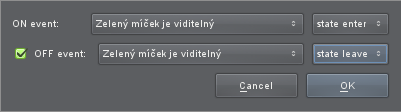
\includegraphics[width=0.8\textwidth]{addswitch.png}
\caption{Přidání nového přepínače}
\label{fig:addswitch}
\end{figure}

Prvním rozbalovacím seznamem vyberete gesto, druhým událost. Pokud k zapínací
události existuje logicky události opačná (např. \emph{stav začal platit} a
\emph{stav přestal platit}), je rozumné ji přidat jako vypínací událost.
Samozřejmě záleží čeho chcete dosáhnout. Přepínače fungují tak, že pokud mám
nastaveny obě události, tak po zapnutí první událostí zůstává zapnutý, dokud
ho druhá událost nevypne. Kdežto, pokud vypínací událost nemá, vypne se hned
po proběhnutí kontroly spouštěče, to má smysl převážně u pohybových gest,
protože mají pouze jednu událost.

Pokud chcete některý přepínač změnit, musíte ho odstranit tlačítkem
\emph{Remove switch} a znovu přidat v nové podobě.

\begin{figure}[H]
\centering
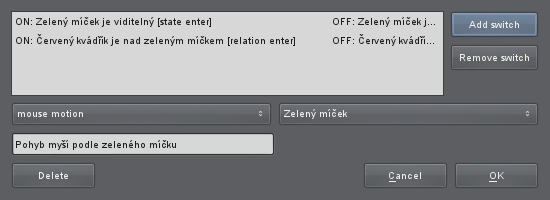
\includegraphics[width=1.1\textwidth]{newactiontrigger.png}
\caption{Přidání nového spoučtěče akce}
\label{fig:newactiontrigger}
\end{figure}

Co se týče akcí, máte na výběr \emph{pohyb myší}, \emph{stisk tlačítek myši} a
\emph{otočení kolečkem}, \emph{stisk klávesy na klávesnici} nebo
\emph{spuštění systémového příkazu}.

\begin{figure}[H]
\centering

\includegraphics[width=1.1\textwidth]{keyaction.png}
\caption{Zadávání akce klávesnice}
\label{fig:keyaction}
\end{figure}

Nastavení akcí myši by mělo být zřejmé. Pozastavíme se u akce stisku klávesy.
Zadání klávesy, které se akce bude týkat probíhá tak, že kliknete na tlačítko
\emph{grab key}. V tu chvílí aplikace čeká na stisk klávesy (viz obrázek
\ref{fig:keyaction}). Skiskněte klávesu na klávesnici a aplikace si ji zaznamená.

Pro zadání systémového příkazu stačí konkrétní příkaz napsat. Jedná se o
jakýkoli příkaz, který lze zapsat do příkazové řádky systému.

\subsection{Testování gest}
Před tím, než spustíte samotné ovládání, je vhodné si nejprve otestovat, zda
vše funguje tak, jak předpokládáte. Můžete testovat buď jednotlivá gesta
kliknutím na tlačítko \emph{Test gesture} v dialogu pro přidávání gesta, nebo
můžete otestovat všechny najednou. Nástroj pro testování všech najednou
naleznete v nabídce \emph{Tools} pod položkou \emph{Test control}.

\begin{figure}[H]
\centering
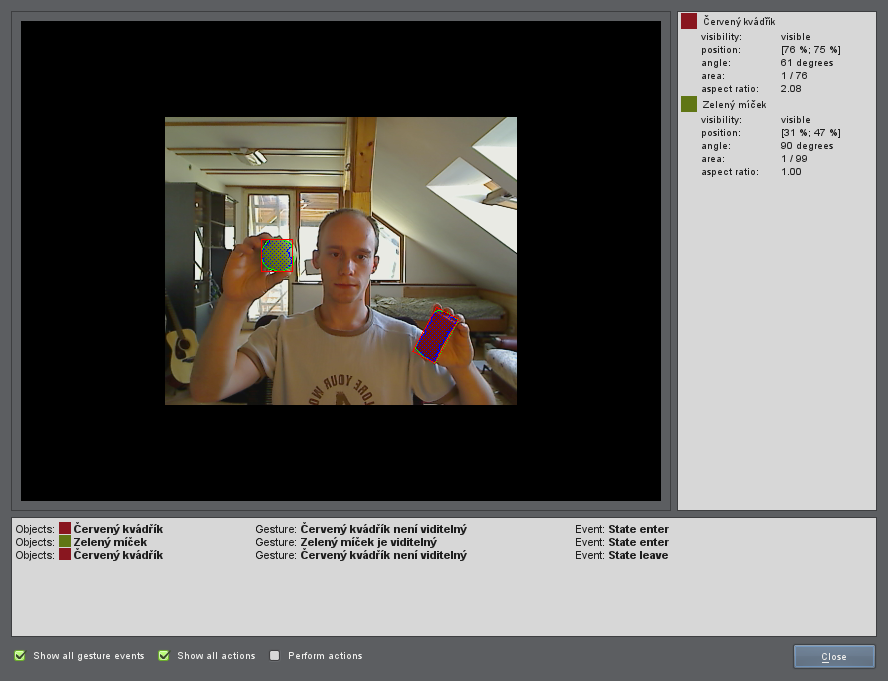
\includegraphics[width=1.1\textwidth]{testgestures.png}
\caption{Testování gest}
\label{fig:testgestures}
\end{figure}

Dialog poskytuje spoustu užitečných informací. Vpravém sloupci zobrazje
aktuální hodnoty vlastnosí objektů. Toho lze využít při navrhování gest, není
třeba vymýšlet z hlavy konkrétní hodnoty pro podmínky.

V dolní části jsou zobrazeny události, které tak jak nastávají za sebou.

Úplně dole je několik zaškrtávacích políček. \emph{Show all gesture events}
zajistí aby byli zobrazeny událost všech gest (smysl má při testování
jednotlivých gest, ve výchozím stavu se totiž zobrazují pouze události
testovaného gesta). \emph{Show all actions} zajistí, aby se zobrazovaly akce
pokud nastanou potřebné události, akce se ale neprovedou, pouze se zobrazí
informace, že by se za normálních okolností v ten okamžik provedly. Pokud ale
chcete akce i provádět, zaškrtněte poslední políčko \emph{Perform actions}.

\subsection{Ovládání}
Nyní je vše připraveno pro samotné ovládání. Spustíte ho tlačítkem \emph{Start
control} ve hlavním okně. Nyní se již nebudou nikde rozbrazovat žádné
informace. Aplikaci je možné dát stranou (minimalizovat, přesunout na jinou
plochu, ...). Ukončení ovládání se provede stejným tlačítkem.


%%% Tabulky v bakalářské práci, existují-li.
%\chapter*{Seznam tabulek}
%\addcontentsline{toc}{chapter}{Seznam tabulek}

%%% Použité zkratky v bakalářské práci, existují-li, včetně jejich vysvětlení.
%\chapter*{Seznam použitých zkratek}
%\addcontentsline{toc}{chapter}{Seznam použitých zkratek}

%%% Přílohy k bakalářské práci, existují-li (různé dodatky jako výpisy programů,
%%% diagramy apod.). Každá příloha musí být alespoň jednou odkazována z vlastního
%%% textu práce. Přílohy se číslují.
%\chapter*{Přílohy}
%\addcontentsline{toc}{chapter}{Přílohy}

\openright
\end{document}
